% generated by scripts/pkl_to_latex.py
% source PKL : uscan_v1_L6_Ne6_t1_mode-uniform_nmin2_solver-gcg_sz0_restarts10_iter200_kmax4_tol1em09_U1to20_N20-d03a74da789e.pkl
% scan type  : uscan
% state      : gs
% quantity   : linear-entropy
% requires   : \usepackage{pgfplots} \pgfplotsset{compat=1.18}
% colours match the matplotlib PDF (tab10 cycle)
\definecolor{gmeC0}{HTML}{1F77B4}
\definecolor{gmeC1}{HTML}{FF7F0E}
\definecolor{gmeC2}{HTML}{2CA02C}
\definecolor{gmeC3}{HTML}{D62728}
\definecolor{gmeC4}{HTML}{9467BD}
\definecolor{gmeC5}{HTML}{8C564B}
\definecolor{gmeC6}{HTML}{E377C2}
\definecolor{gmeC7}{HTML}{17BECF}

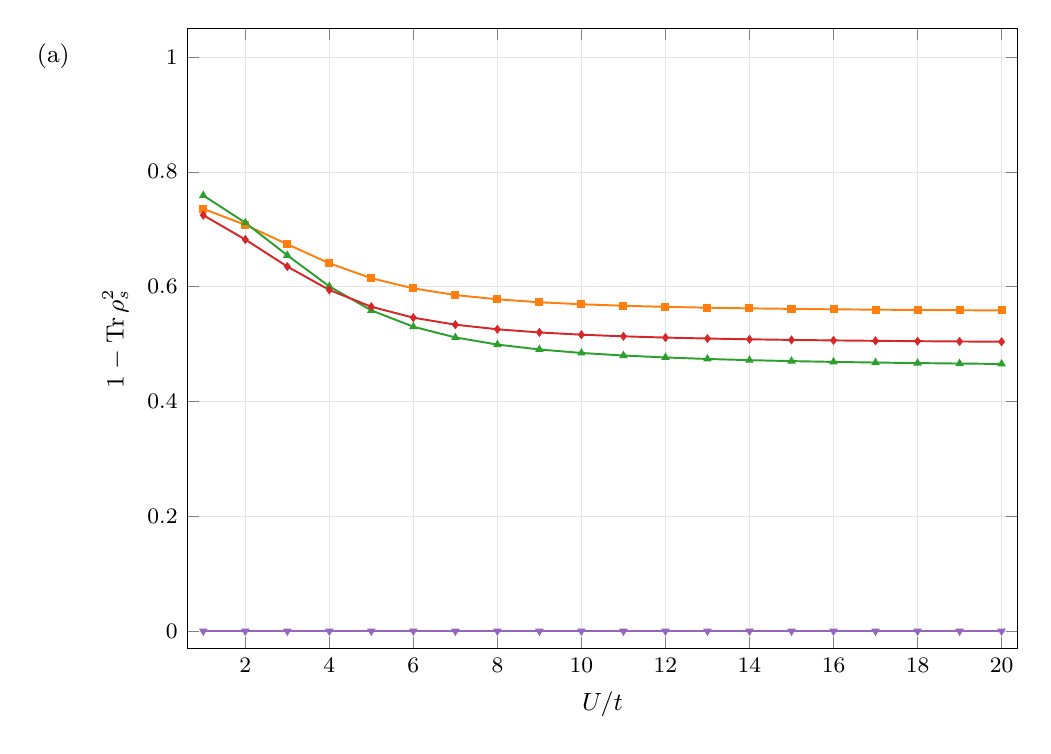
\begin{tikzpicture}
  \begin{axis}[
    width=\columnwidth,
    height=0.78\columnwidth,
    xlabel={$U/t$},
    ylabel={$1-\mathrm{Tr}\,\rho_s^2$},
    grid=both,
    grid style={line width=.1pt, draw=gray!20},
    tick label style={font=\footnotesize\rmfamily, /pgf/number format/fixed},
    label style={font=\small\rmfamily},
    scaled ticks=false,
    legend style={font=\scriptsize\rmfamily, draw=gray!40, at={(0.5,1.03)}, anchor=south, /tikz/every even column/.append style={column sep=6pt}},
    legend cell align={left},
    legend columns=2,
    ymin=-0.03,
    ymax=1.05,
    xmin=0.62,
    xmax=20.38,
    after end axis/.append code={\node[anchor=east, font=\small\rmfamily] at (axis description cs:-0.13,0.954) {(a)};},
  ]
    \addplot[color=gmeC1, mark=square*, mark size=1.1pt, line width=0.7pt] coordinates {
        (1,0.735414) (2,0.707688) (3,0.67383) (4,0.640678)
        (5,0.61465) (6,0.596903) (7,0.585393) (8,0.577874)
        (9,0.572807) (10,0.569263) (11,0.566697) (12,0.564781)
        (13,0.563312) (14,0.562161) (15,0.561241) (16,0.560493)
        (17,0.559878) (18,0.559365) (19,0.558933) (20,0.558565)
    };
    \addplot[color=gmeC2, mark=triangle*, mark size=1.1pt, line width=0.7pt] coordinates {
        (1,0.75883) (2,0.711312) (3,0.654537) (4,0.600411)
        (5,0.558648) (6,0.530199) (7,0.511523) (8,0.4991)
        (9,0.490564) (10,0.484489) (11,0.480021) (12,0.47664)
        (13,0.474021) (14,0.471949) (15,0.470282) (16,0.468919)
        (17,0.467791) (18,0.466847) (19,0.466048) (20,0.465366)
    };
    \addplot[color=gmeC3, mark=diamond*, mark size=1.1pt, line width=0.7pt] coordinates {
        (1,0.724443) (2,0.682011) (3,0.635001) (4,0.594188)
        (5,0.564959) (6,0.545932) (7,0.533732) (8,0.525704)
        (9,0.520215) (10,0.516315) (11,0.513449) (12,0.511281)
        (13,0.509601) (14,0.508272) (15,0.507202) (16,0.506328)
        (17,0.505605) (18,0.504999) (19,0.504487) (20,0.504049)
    };
    \addplot[color=gmeC4, mark=triangle*, mark size=1.1pt, mark options={rotate=180}, line width=0.7pt] coordinates {
        (1,-0) (2,0) (3,-0) (4,0)
        (5,0) (6,-0) (7,0) (8,-0)
        (9,0) (10,0) (11,0) (12,0)
        (13,-0) (14,-0) (15,0) (16,-0)
        (17,0) (18,0) (19,-0) (20,0)
    };
  \end{axis}
\end{tikzpicture}
